\newpage
\section{Configurazione}
\rhead{Configurazione}
\subsection{Struttura del package di lancio}
\label{sub:strpackage} 
Per il corretto funzionamento del tool risulta fondamentale strutturare in modo corretto il package di lancio (Figura \ref{fig:strdir}) in modo da permettere una corretta lettura dei file di configurazione e dei file di input.

\begin{figure}[H]
	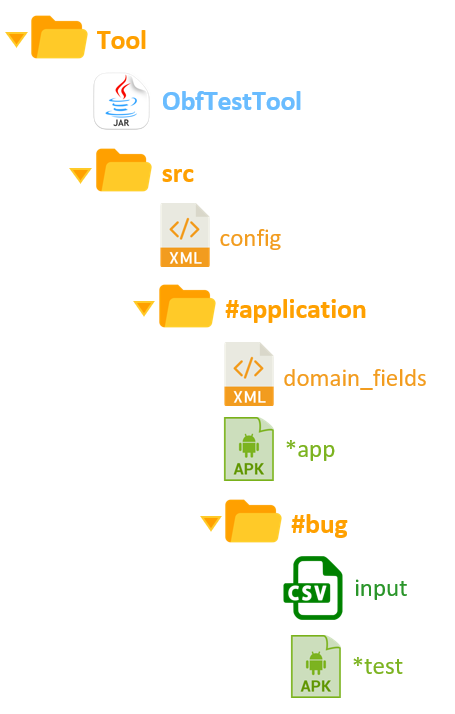
\includegraphics[scale=0.55]{struttura.directory}
	\centering
	\caption{Struttura package di lancio}%\footnote{Immagine realizzata da A. Belisario}
    \label{fig:strdir}
\end{figure}


\noindent La struttura del package di lancio prevede la possibilità di:
 \begin{itemize} [nosep]	
		\item inserire nella cartella 'src' più cartelle '\#application'
		\begin{description}[nosep]
    		 \item \emph{(il tool permette di tenere in memoria più applicazioni)}
    	\end{description}
		\item inserire nella cartella '\#application' più cartelle '\#bug'
		\begin{description}[nosep]
    		 \item \emph{(il tool permette di tenere in memoria più bug per applicazione)}
    	\end{description}
\end{itemize}
\noindent Nella struttura del package il nome dei file e delle cartella è vincolante, con alcune eccezioni:
 \begin{itemize} [nosep]	
		\item alle cartelle il cui nome nella Figura \ref{fig:strdir} inizia con il carattere '\#' dovrà essere attributo un nome significativo
		\item  il nome dei file il cui nome nella Figura \ref{fig:strdir} inizia con il carattere '\mbox{*}' è indifferente al funzionamento del tool
		\item il nome della cartella radice, chiamata nella Figura \ref{fig:strdir}  'Tool', è indifferente al funzionamento del tool
\end{itemize}
L'architettura della soluzione e le scelte strutturali effettuate per il package di lancio possono essere comprese maggiormente andando ad analizzare brevemente l'utilità dei singoli file:

\begin{tcolorbox} [colback=white, colframe=lightgray]
 	
\includegraphics[height=1cm]{icona.jar} \newline
File JAR lanciabile da linea di comando in cui è stato impacchettato il tool che offre diverse funzionalità. Comprende al suoi interno anche la libreria di offuscamento.
\end{tcolorbox}
	
\begin{tcolorbox}[colback=white, colframe=lightgray]
	 
\includegraphics[height=1cm]{icona.config} \newline
File di configurazione dell'intero tool contenente parametri utili all'offuscamento dei dati e all'automazione dei test. I parametri nel file sono definiti in modo differenziato per ogni bug di ogni applicazione. 
\end{tcolorbox}

\begin{tcolorbox}[colback=white, colframe=lightgray]
	 
\includegraphics[height=1cm]{icona.domain} \newline
File xml contenente i domini dei campi dell'applicazione utili alla libreria di offuscamento nell'applicazione delle tecniche.
\end{tcolorbox}

\begin{tcolorbox}[colback=white, colframe=lightgray]
	 
\includegraphics[height=1cm]{icona.input} \newline
File csv contenente le tuple da offuscare. Ai fini dello stage saranno inserite le tuple che generano il bug.
\end{tcolorbox}

\begin{tcolorbox}[colback=white, colframe=lightgray]
	 
\includegraphics[height=1cm]{icona.app} \newline
File APK dell'applicazione da testare.
\end{tcolorbox}

\begin{tcolorbox}[colback=white, colframe=lightgray]
	 
\includegraphics[height=1cm]{icona.test} \newline
File APK di test dell'applicazione da testare che permette il lancio del caso di test parametrico che dovrebbe riprodurre il bug.
\end{tcolorbox}

\subsection{File di configurazione e file di input}
\label{fileconfigfileinput}
I file di configurazione e i file di input, come spiegato nella sezione precedente (Sezione \ref{sub:strpackage}), sono essenziali al funzionamento del tool e richiedono di essere prodotti rispettando alcuni restringenti requisiti.  

\subsection*{File di input dei dati \textcolor{gray}{input.csv} }   
\label{filediinputdeidati}
Il file \emph{input.csv} contiene il dataset dei valori inseriti nell'applicazione dall'utente, idealmente ricavati dal log di esecuzione. Le tuple contenute sono destinate ad essere totalmente o in parte offuscate, in base ai parametri del file di configurazione. 

\noindent Il file deve essere in formato csv in modo da essere facilmente leggibile (se aperto con un CSV viewer i dati vengono incolonnati come in Figura  \ref{fig:csvviewer}) e facile da modificare sia dall'utente che dal tool. Il file deve rispettare un pattern semplice: 

 \begin{itemize} [nosep]	
		\item[] \textbf{prima riga } \quad nomi/etichette delle colonne/campi  divise da un ';'
		\item[] \textbf{righe successive } \quad tupla di valori ordinati delle colonne/campi divisi da un ';
\end{itemize}
\noindent La figura  \ref{fig:csvtext}  mostra l'esempio di un file di input dei dati in cui il pattern è rispettato.

\begin{figure}[H]
    \centering
    \begin{minipage}{0.4\textwidth}
        \centering
        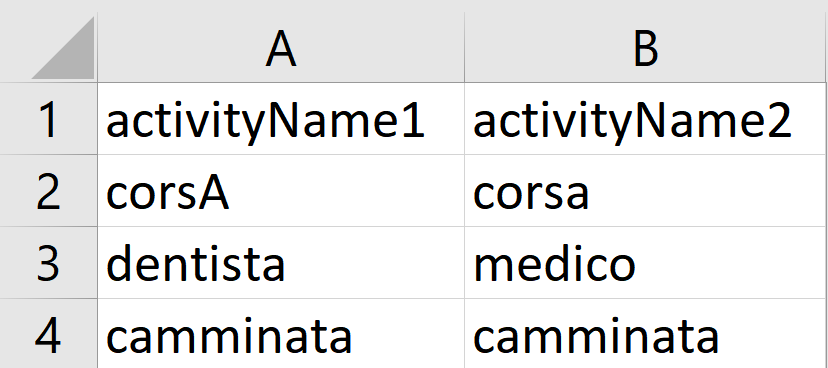
\includegraphics[width=4cm]{csv.viewer} 
        \caption{File di input (viewer)}
            \label{fig:csvviewer}
    \end{minipage}\hfill
    \begin{minipage}{0.6\textwidth}
        \centering
        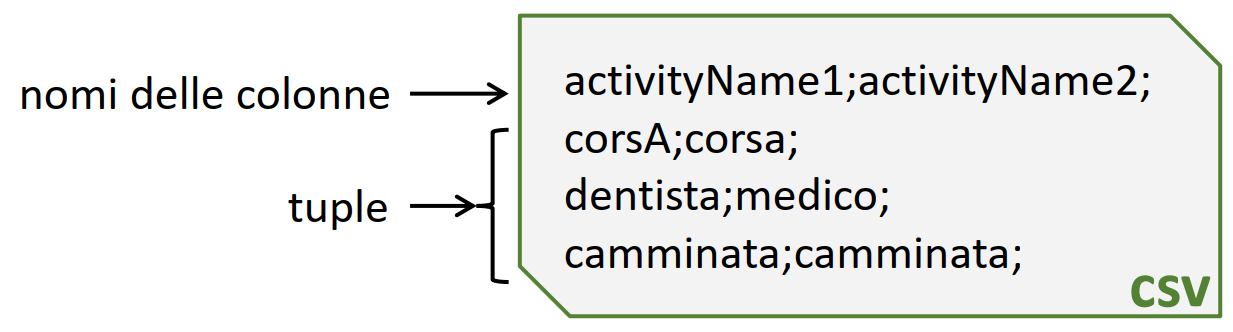
\includegraphics[width=8cm]{csv.text} 
        \caption{File di input (pattern)}
            \label{fig:csvtext}
    \end{minipage}
\end{figure}


\subsection*{File di configurazione generale \textcolor{gray}{config.xml} }
\label{filconfiggeneral}
Il file di configurazione generale permette di parametrizzare in modo semplice l'applicativo, con informazioni che riguardano sia l'offuscamento dei dati che l'automazione dei test (e conseguente verifica della riproduzione del bug atteso). I parametri nel file sono definiti in modo differenziato per ogni bug di ogni applicazione.  Il file di configurazione deve esser in formato xml e deve rispettare una struttura ben precisa.
\begin{figure}[H]
	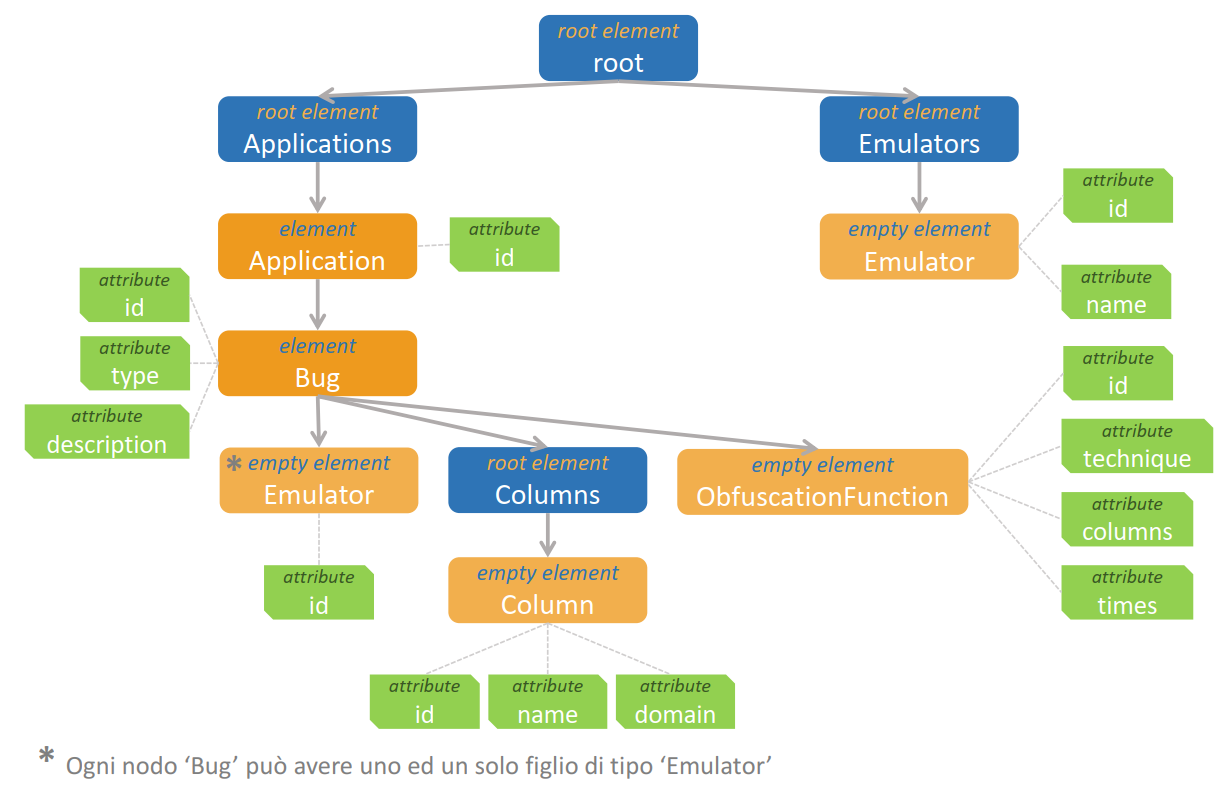
\includegraphics[scale=0.55]{tree.structure}
	\centering
	\caption{Struttura ad albero del file xml di configurazione}%\footnote{Immagine realizzata da A. Belisario}
    \label{fig:configstructure}
\end{figure}
\noindent Il pattern richiesto dal documento è schematizzato in  Figura \ref{fig:configstructure}: la struttura dell'albero xml può essere compresa nei dettagli solo conoscendo le varie tipologie di nodo/attributo (Appendice A - Lettura degli alberi xml).


\noindent Per sfruttare a pieno le potenzialità del tool (utilizzare sia le funzionalità di offuscamento che di automazione) è necessario compilare il file di configurazione in ogni sua parte e non tralasciare quindi nessun nodo e nessun attributo dell'albero. 

\noindent La correlazione tra la struttura del package di lancio (Figura \ref{fig:strdir}) e la struttura del file xml (Figura \ref{fig:configstructure}) è molto forte per ovvi motivi. Le scelte strutturali effettuate per il file di configurazione potrebbero essere comprese maggiormente andando ad analizzare l'utilità dei singoli nodi e dei relativi attributi:
 \begin{itemize} [nosep]	
		\item[$\blacksquare$] \textbf{root}  \newline
		Il nodo 'root' è il nodo radice dell'albero. Non svolge una funzionalità particolare, se non quella di permettere il rispetto delle regole previste dallo standard xml, che impone di avere un singolo nodo radice nel documento. 
		\item[$\blacksquare$] \textbf{Applications}  \newline
		Il nodo 'Applications' è il nodo genitore di tutte le applicazioni. 
			\item[$\blacksquare$] \textbf{Application}  \newline
		I nodi 'Application' rappresentano le applicazioni Android. 
		 \begin{itemize} [nosep]	
		\item \textbf{id} L'attributo rappresenta l'id con cui si vuole memorizzare l'applicazione. Il valore di questo campo deve corrispondere al nome della relativa cartella nel package di lancio, indicata nella Figura \ref{fig:strdir} con '\#application'  (join).
		\end{itemize}
		\item[$\blacksquare$] \textbf{Bug}  \newline
		I nodi 'Bug' rappresentano i bug delle applicazioni  sui  quali si vogliono sfruttare le funzionalità del tool. Per come è strutturato il file di configurazione, per ogni applicazione possono essere inseriti più bug.
		 \begin{itemize} [nosep]	
		\item \textbf{id} L'attributo rappresenta l'id con cui si vuole memorizzare il bug. Il valore di questo campo deve corrispondere al nome della relativa cartella nel package di lancio, indicata nella Figura \ref{fig:strdir} con '\#bug' (join).
			\item \textbf{type} L'attributo è opzionale e rappresenta il tipo di bug atteso. Può assumere uno tra i valori 'assertion', 'exception', 'crash' o  'NS'. L'attributo influsce sulla valutazione della riproduzione del bug atteso, che viene trattata nella Sezione \ref{valbugatt}.
			\item \textbf{description} L'attributo è opzionale e rappresenta la descrizione testuale del bug atteso.
		\end{itemize} 
			\item[$\blacksquare$] \textbf{Emulator} (figlio del nodo 'Bug')  \newline
		Il nodo 'Emulator' rappresenta l'emulatore su cui lanciare i test. 
			 \begin{itemize} [nosep]	
		\item \textbf{id} L'attributo rappresenta l'id dell'emulatore su cui lanciare i test.  Il valore di questo campo deve corrispondere con l'id di uno dei nodi Emulator figli del nodo Emulators (join).
			\end{itemize} 
			\item[$\blacksquare$] \textbf{Columns}  \newline
		Il nodo 'Columns' è il nodo genitore delle colonne del file di input. 
	\item[$\blacksquare$] \textbf{Column}  \newline
		I nodi 'Column' rappresentano le colonne/i campi del file di input. Per ogni colonna del file \emph{input.csv}, deve essere presente un nodo con tag 'Column'.
		 \begin{itemize} [nosep]	
		\item \textbf{id} L'attributo rappresenta l'id numerico della colonna. 
		\item  \textbf{name} L'attributo rappresenta il nome della colonna.  Il valore di questo campo deve corrispondere con il relativo nome della colonna nel file \emph{input.csv}.
		\item  \textbf{domain} L'attributo rappresenta l'id numerico del dominio del campo.  Il valore dell'attributo deve corrispondere con l'id di uno dei domini configurati nel file \emph{domain\_fields.xml}. 
			\end{itemize} 
			\item[$\blacksquare$] \textbf{ObfuscationFunction}  \newline
		I nodi 'ObfuscationFunction' rappresentano le funzioni di offuscamento applicabili.
		 \begin{itemize} [nosep]	
		\item \textbf{id} L'attributo rappresenta l'id della funzione di offuscamento. 
		 		\item \textbf{technique} L'attributo rappresenta il nome letterale della tecnica di offuscamento. Serve per invocare la corretta funzione nella
libreria delle tecniche di offuscamento ('localSuppression', 'generalization'...).
		\item \textbf{columns} L'attributo rappresenta gli id delle colonne da offuscare, separati dal ';'. 
		\item \textbf{times} L'attributo rappresenta il numero di volte di applicazione della tecnica di offuscamento sui dati. 
			\end{itemize} 
			\item[$\blacksquare$] \textbf{Emulators}  \newline
		Il nodo 'Emulators' è il nodo genitore di tutti gli emulatori.
		\item[$\blacksquare$] \textbf{Emulator} (figlio del nodo 'Emulators') \newline
		I nodi 'Emulator' rappresentano gli emulatori assegnabili ai vari bug.
		 \begin{itemize} [nosep]	
				\item \textbf{id} L'attributo rappresenta l'id dell'emulatore. 
		 		\item \textbf{name} L'attributo rappresenta il nome dell'emulatore.   Il valore di questo campo deve corrispondere con il nome di uno degli AVD\footnote{\textbf{AVD}: Android Virtual Device, configurazione che definisce le caratteristiche di un dispositivo che si vuole simulare} configurati (Appendice A - Configurazione degli AVD).
			\end{itemize} 
\end{itemize}
\begin{figure}[H]
	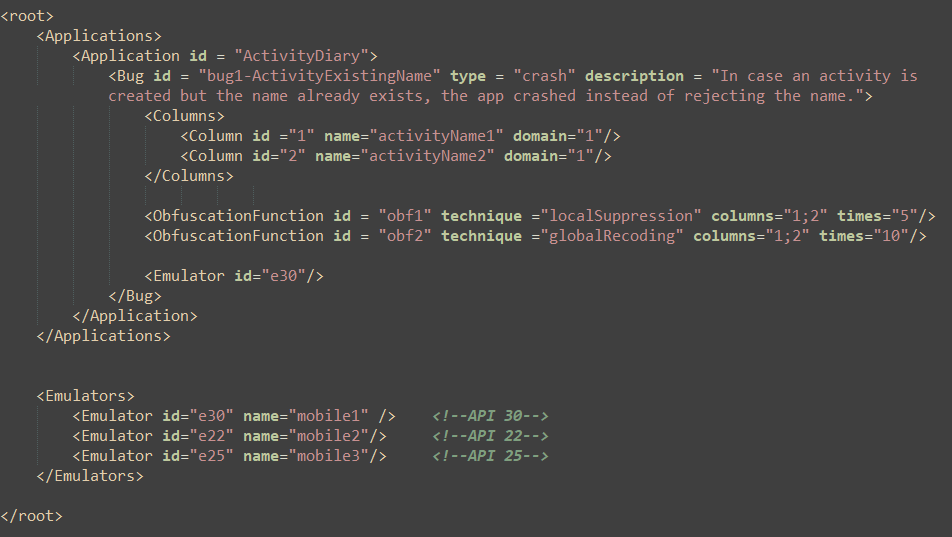
\includegraphics[scale=0.55]{config.example}
	\centering
	\caption{Esempio: \emph{config.xml}}
    \label{fig:configexample}
\end{figure}
Nella Figura \ref{fig:configexample} viene mostrato lo screenshot di un file di configurazione correttamente impostato.


\subsection*{File di configurazione dei domini \textcolor{gray}{domain\_fields.xml}}
Il file di configurazione dei domini ha il fine di contenere i domini dei campi dell'applicazione, utili alla libreria nell'applicazione delle tecniche di offuscamento. Ogni nodo 'Column' del file di configurazione generale infatti, come analizzato nella sezione precedente (Sezione \ref{filconfiggeneral}), ha un attribito dominio il cui valore deve corrispondere all'identificativo di un dominio nel relativo file \emph{domain\_fields.xml}. Il documento è stato strutturato in maniera completamente identica a quella prevista dal collega A. Belisario nella sua tesi magistrale. 
\begin{figure}[H]
	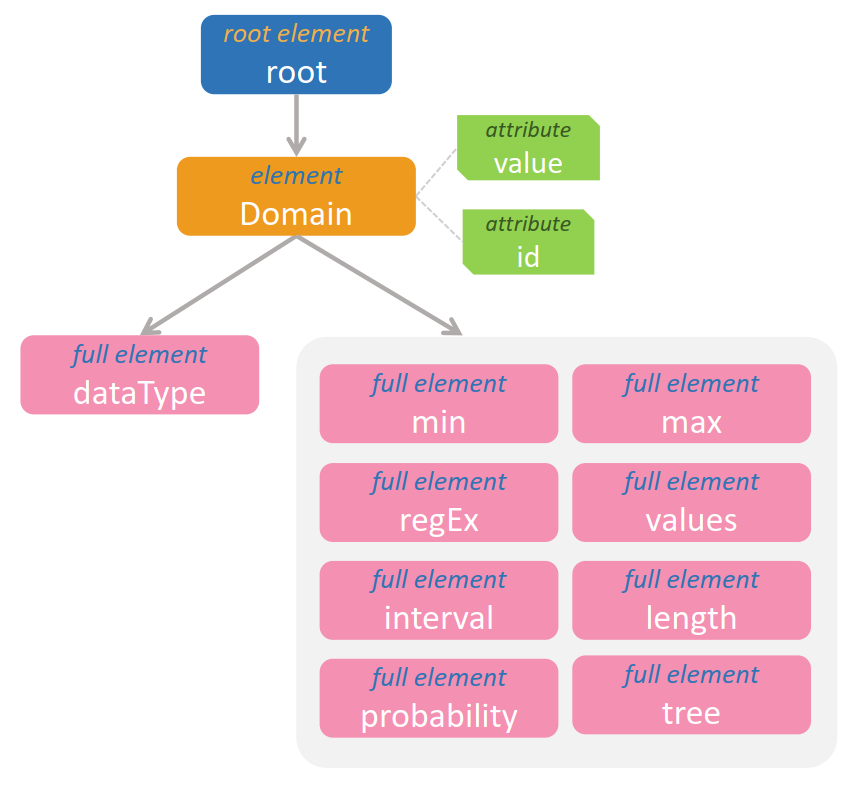
\includegraphics[scale=0.45]{domain.tree.structure}
	\centering
	\caption{Struttura ad albero del file xml di configurazione}%\footnote{Immagine realizzata da A. Belisario}
    \label{fig:domainconfigstructure}
\end{figure}
\noindent La struttura dell'albero xml (Figura \ref{fig:domainconfigstructure}) può essere compresa nei dettagli solo conoscendo le varie tipologie di nodo/attributo (Appendice A - Lettura degli alberi xml). La struttura del file è dinamica in base:
\begin{itemize} [nosep]
\item [-]  alle informazioni necessarie per definire il dominio del dato
\item [-]  alle informazioni necessarie ad ogni tecnica per poter offuscare nel modo corretto
\end{itemize}
Per quanto rigurda il dominio del dato, solo il  nodo 'dataType' è  sempre obbligatorio, mentre l'obbligatorietà degli altri nodi dipende dal suo valore:
\begin{itemize}[nosep]
\item dataType=\textbf{Continuous}
\begin{itemize}[nosep]
\item\textbf{min}  valore limite inferiore dell’insieme
\item\textbf{max}  valore limite superiore dell’insieme
\end{itemize}
\item dataType=\textbf{Categorical}
\begin{itemize}[nosep]
\item\textbf{values}  lista dei valori che il campo può assumere, separati da un ';'
\end{itemize}
\item dataType=\textbf{StringType}
\begin{itemize}[nosep]
\item\textbf{regEx}  espressione regolare che definisce il dominio del campo
\item\textbf{length}  numero che definisce la lunghezza della stringa in output, se viene indicato il carattere ’=’ questa sarà generata con una lunghezzauguale a quella passata in input
\end{itemize}
\end{itemize}
\noindent Per quanto rigurda le informazioni necessarie alla tecnica di offuscamento, possono essere definiti i nodi:
\begin{itemize}[nosep]
\item \textbf{tree}  albero di gerarchia (indicando con root il valore più generico e ricorsivamente attraverso il tag node tutti i figli)
\item \textbf{probability} matrice N*N (N sono i possibili valori che assume la variabile)
\end{itemize}
\begin{figure}[H]
	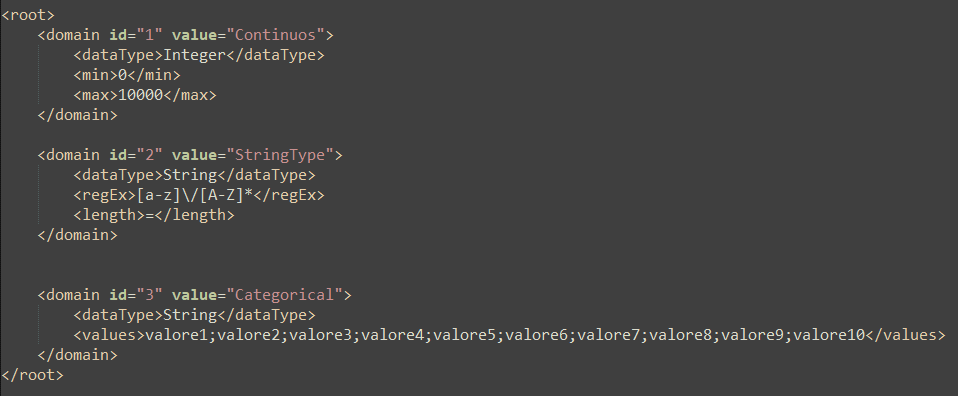
\includegraphics[scale=0.6]{domain.example}
	\centering
	\caption{Esempio: \emph{domain.xml}}
    \label{fig:domainexample}
\end{figure}
Nella Figura \ref{fig:domainexample} viene mostrato lo screenshot di un file di configurazione dei domini correttamente impostato.

\subsection*{File APK \textcolor{gray}{app.apk, test.apk}}   
La generazione dei file \emph{app.apk} e \emph{test.apk} implica l'esecuzione di diversi passaggi  che possono variare in base a differenti fattori (uno tra tutti la disponibilità del codice sorgente dell'applicazione). Per questo motivo il tema verrà trattato in un capitolo a parte (Capitolo \ref{genapk}).